\documentclass{sigchi-ext}
% Please be sure that you have the dependencies (i.e., additional
% LaTeX packages) to compile this example.
\usepackage[T1]{fontenc}
\usepackage{textcomp}
\usepackage[scaled=.92]{helvet} % for proper fonts
\usepackage{graphicx} % for EPS use the graphics package instead
\usepackage{balance}  % for useful for balancing the last columns
\usepackage{booktabs} % for pretty table rules
\usepackage{ccicons}  % for Creative Commons citation icons
\usepackage{ragged2e} % for tighter hyphenation

% Some optional stuff you might like/need.
% \usepackage{marginnote}
% \usepackage[shortlabels]{enumitem}
% \usepackage{paralist}
% \usepackage[utf8]{inputenc} % for a UTF8 editor only

%% OVERRIDE THE DEFAULT COPYRIGHT STRIP
\copyrightinfo{Permission to make digital or hard copies of part or all of this work for personal or classroom use is granted without fee provided that copies are not made or distributed for profit or commercial advantage and that copies bear this notice and the full citation on the first page. Copyrights for third-party components of this work must be honored. For all other uses, contact the Owner/Author.\\
Copyright is held by the owner/author(s).\\
{\emph{TEI'17}}, March 20-23, 2017, Yokohama, Japan.\\
ACM XXX-X-XXXX-XXXX-X/XX/XX\\
\url{http://dx.doi.org/XX.XXXX/XXXXXXX.XXXXXXX}}

% Paper metadata (use plain text, for PDF inclusion and later
% re-using, if desired).  Use \emtpyauthor when submitting for review
% so you remain anonymous.
\def\plaintitle{Musical Skins: Fabric Interfaces for Expressive Music Control}
\def\plainauthor{Maurin Donneaud, Cedric Honnet, Paul Strohmeier}
\def\emptyauthor{}
\def\plainkeywords{Musical Interface, e-Textile, soft circuits, on-body interaction}
\def\plaingeneralterms{Documentation, Standardization}

\title{Musical Skins: Fabric Interfaces for Expressive Music Control}

\numberofauthors{3}
% Notice how author names are alternately typesetted to appear ordered
% in 2-column format; i.e., the first 4 autors on the first column and
% the other 4 auhors on the second column. Actually, it's up to you to
% strictly adhere to this author notation.
\author{%
    % use left blank space to show an overview of the project
    \makebox(-36,-175){ 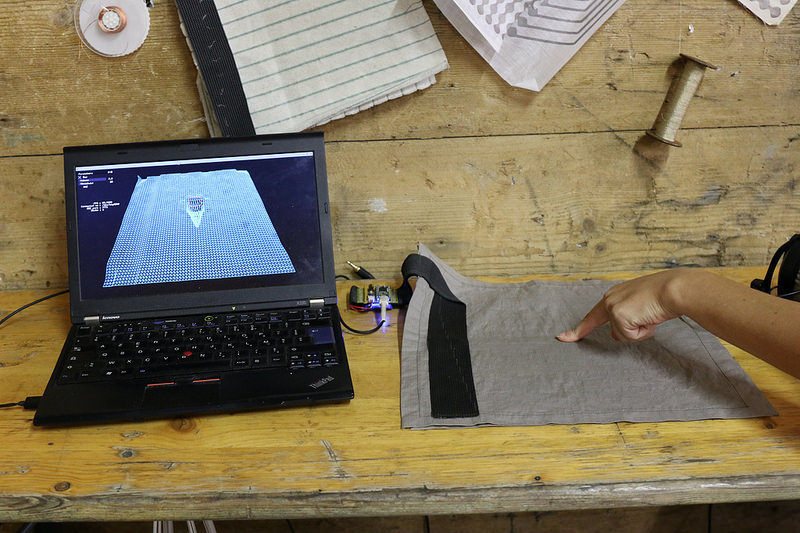
\includegraphics[width=1.05\columnwidth]{figures/touch} }
    \alignauthor{~}
    \alignauthor{~}
    \alignauthor{%
        \textbf{Maurin Donneaud}\\
        \affaddr{DataPaulette} \\
        \affaddr{France} \\
        \email{firstname@institution.org} \\
        \textbf{~} \\
        \textbf{~} \\
    }
    \alignauthor{~}
    \alignauthor{%
        \textbf{Cedric Honnet}\\
        \affaddr{CarpeNoctem} \\
        \affaddr{France} \\
        \email{firstname@institution.cc} \\
        \textbf{~} \\
        \textbf{~} \\
    }
    \alignauthor{~}
    \alignauthor{%
        \textbf{Paul Strohmeier}\\
        \affaddr{University of Copenhagen} \\
        \affaddr{Denmark} \\
        \email{firstname.lastname@gmail.com}
    }
    % caption of the picture
    \makebox(-80,-30){ \textbf{Figure 0:} Visualization of the Musical Skin being touched.}
}

% Make sure hyperref comes last of your loaded packages, to give it a
% fighting chance of not being over-written, since its job is to
% redefine many LaTeX commands.
\definecolor{linkColor}{RGB}{6,125,233}
\hypersetup{%
  pdftitle={\plaintitle},
  pdfauthor={\plainauthor},
  pdfkeywords={\plainkeywords},
  bookmarksnumbered,
  pdfstartview={FitH},
  colorlinks,
  citecolor=black,
  filecolor=black,
  linkcolor=black,
  urlcolor=linkColor,
  breaklinks=true,
}

% \reversemarginpar%

\begin{document}

\maketitle

% Uncomment to disable hyphenation (not recommended)
% https://twitter.com/anjirokhan/status/546046683331973120
\RaggedRight{}

% Do not change the page size or page settings.
\begin{abstract}
We present an installation consisting of three soft, malleable fabric instruments. Visitors can use these instruments to explore sounds, collaboratively create soundscapes and music, as well as control the ambient lighting. Our soft instruments - musical skins - sense where they are touched and how much pressure is exerted on them. This is done using a novel sensing method consisting entirely of fabric components. In this extended abstract we discuss the sensing mechanism and describe the installation we envision our musical skins to be used in.
\end{abstract}

\keywords{\plainkeywords}

\category{H.5.m}{Information interfaces and presentation}{Miscellaneous}
\category{J.5}{Arts and humanities}{Arts, fine and performing.}

\section{Introduction}
We present an art installation using Musical Skins: soft, malleable fabric interfaces that users can freely manipulate to play music. Musical Skins can be draped over objects, worn, folded, pulled, bent and squished to produce sound. If worn draped over the body - as a scarf, cape, skirt, bracelet - interesting feedback modalities emerge. The users feel the tactile properties of the fabric in their fingertips, while at the same time feeling the pressure and taps of the fingers through their body. Additionally percussive hits, tones and pads fill the room with sound, leading to a multisensory experience involving the entire body.

We are currently bombarded with advertisement telling us to buy the next wearable gadget to be fitter, happier, more productive. However, these devices are typically rigid both in their form and their expression. Their rigid form does not conform to the bodies soft and dynamic shapes, while their functions are typically constrained by a world view focused on productivity and optimization.

Like the wearable technologies currently pushed by large companies, our fabric can also be worn, but instead of helping us to reach our next goal faster and more efficiently, our fabric invites us to rest and explore our bodies. As it is soft, it can conform to the shape of the body in different ways. By manipulating the material draped over our bodies, we explore ourselves, while creating an audible, shared musical experience. We designed our fabric for pleasure and self-expression, opposing a view of ubiquitous computing that turns us into productivity machines.

We present three different Musical Skins. These mimic the typical composition of a modern pop band. One Skin is an imitation of a drum kit, enabling users to create distinct beats and one-shot sounds by tapping it. Another represents a lead instrument: touching it creates distinct tones. Depending on the touch, the sound spectrum and pitch of the tone changes, allowing users to play haunting melodies on it. A third Skin represents the harmonics section enabling the exploration of different chords and soundscapes, creating a backdrop for the other two instruments to explore. These three instruments will be freely accessible to all visitors during the exhibit. As they are very robust, no special training or instruction is required for visitors.


\section{Related Work}
Electronic textiles have recently received a significant amount of attention with the publication of public Jacquard \cite{jacquard}, however e-textiles and soft circuitry have a much longer history.

Joanna Berzowska presented wearable e-textile fashion in 2004\cite{berzowska:04}, the dresses she designed retained a 'memory' of intimate experiences of the wearer. Berzowska also demonstrated fabric as an output medium in 2004 \cite{berzowska:05} , with a canvas artwork that slowly changed color.

Hannah Perner Wilson published an overview of soft fabric sensors in 2009 \cite{perner-wilson:09} and has since expanded on that work \cite{perner-wilson:10}. She is currently maintaining an archive of soft textile sensors\footnote{\url{http://www.kobakant.at/DIY}}.

Similar resistive sensing solutions to those used by Musical Skins are used as rapid-prototyping methods. Some of these methods have been documented by David Holman \cite{holman:14, holman:11}.

Our musical skins add additinal expressive modaleties over typical keyed input devices. This method has also been explored by others, for example, Seabord and Linnstrument \cite{seaboard, linnstrument} add preassure and position sensing to the individual 'keys' of a keyboard. Lambdoma and Omnichord are instruments that, like our Skins have explored two dimensional key layouts \cite{lambdoma, omnichord}.


\section{History}
The technology used in our textile instruments is based on the work by Maurin Donneaud \cite{donneaud}. Starting in 2005, he was researching the use of textiles as an intuitive way of interact with computers. From the beginning, his aim was to develop technologies with artistic applications: playing music, creating interactive visualizations etc. To achieve this, the tactile properties and affordances of the interface were a primary focus.

Donneaud's sensor is the result of a reflection on the composition and the interpretation of electronic music. A crossover between the world of weaving and electronics. He opted to use textiles, to give a sensual and intuitive dimension to controllers used to play electronic music. Going beyond its original purpose of a musical instrument, his textile sensor acts as an artificial skin which can provide objects with a sense of touch.

The other inspiration for this installation is TapMe \cite{tapme}, a wearable percussive kit designed by Cedric Honnet. Designed in Paris in 2011, TapMe supports beat-boxers and rappers in the expansion of their expressivity by amplifying body percussion. A performer wearing TapMe can create different beats and drum hits by hitting thin drum-triggers worn on their body.


\section{Implementation}

This textile sensor was designed with open source collaborative development in mind. The hardware and software designs are freely available and documented at \url{eTextile.org}. The design consists of the sensor, which is completely made of fabric, a microcontroller and some basic circuitry that sends electrical signals through the fabric sensor and measures how they are influenced by the fabric sensor, a computer application that interprets the data and passes them on as OSC messages


\begin{marginfigure}[-57ex]
  \begin{minipage}{\marginparwidth}
    \centering
    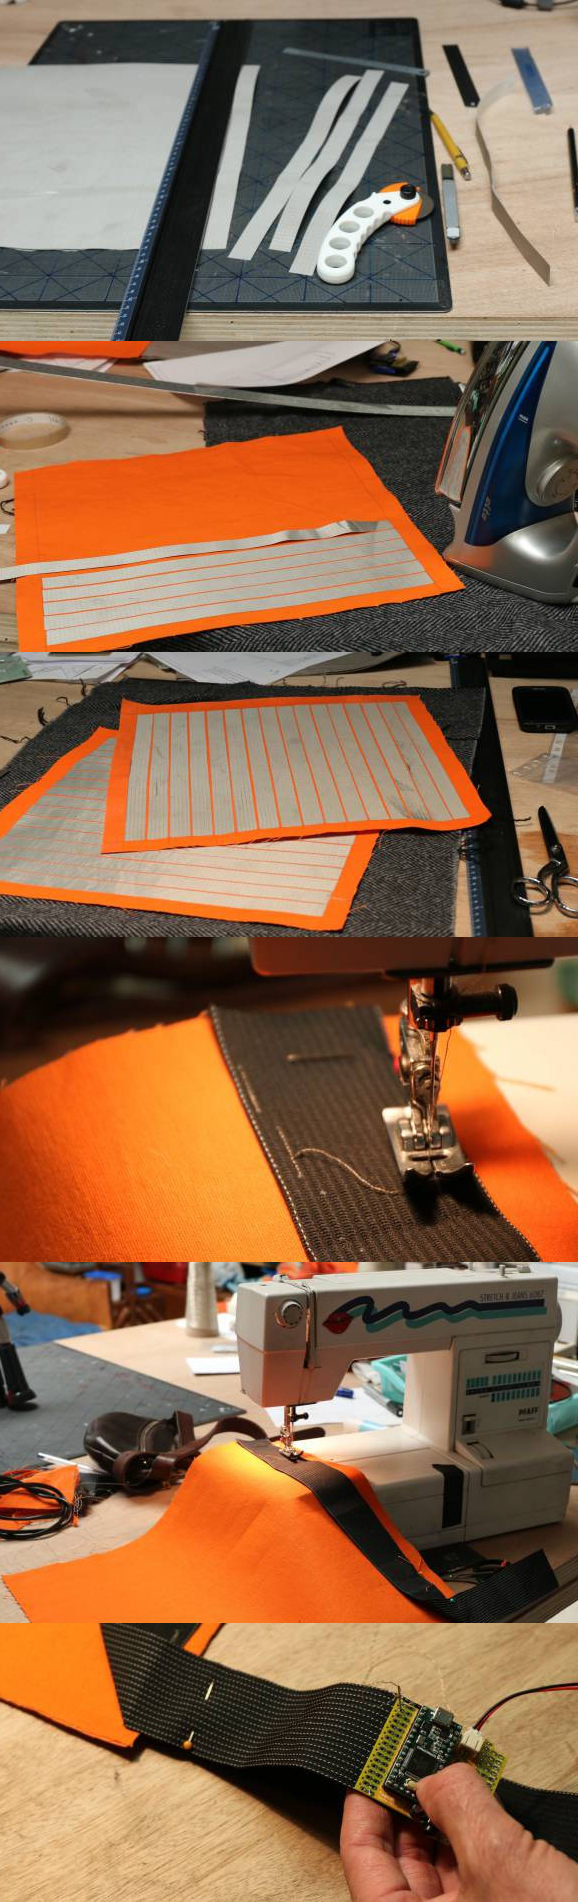
\includegraphics[width=0.9\marginparwidth]{figures/tutorial}
    \caption{Steps to create the conductive layer and connect it to the microcontroller.}~\label{fig:tutorial}
  \end{minipage}
\end{marginfigure}

\subsection{Fabric Sensor}
\subparagraph{Textiles}
The sensor consists of a grid of vertical (x) and horizontal (y) conductive textile strips (see figure \ref{fig:inside}), seperated by a piezoelectric fabric. When the material is touched, the piezoelectrical material is compressed, decreasing its resistance.
To detect position of touch points, we measure the resistance between all strips. If the resistance between two strips drops, we know that the intersection between these two strips is where the touch occurred. We can infer the preassure pressure intensity (z) of this touch, by the magnitude of the change in resistance. We call this combination of x, y and z measurement 3d pressure sensing.

\begin{figure}[h!]
    \centering
    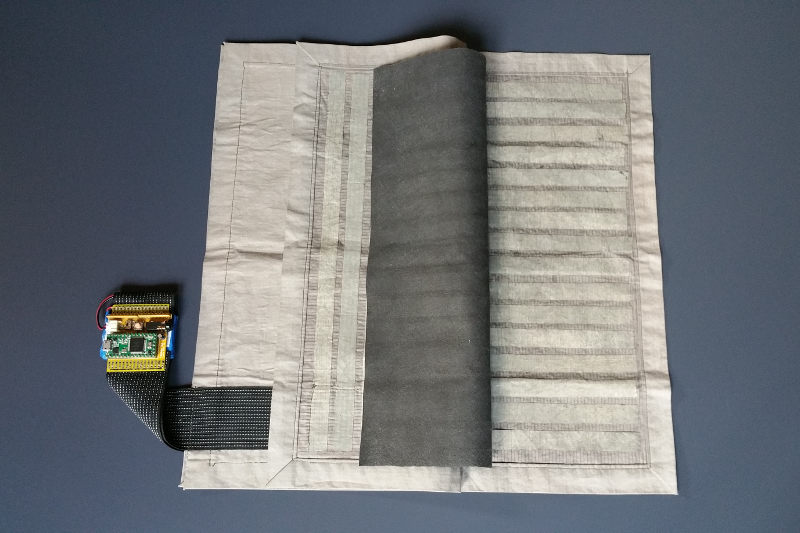
\includegraphics[width=\columnwidth]{figures/inside}
    \caption{The vertical and horizontal stripes of conductive fabric,
    and the resistive fabric in the middle (dark grey).}\label{fig:inside}
\end{figure}

The conductive fabric used is made by stratex \footnote{\url{http://statex.de}} but there are many affordable alternatives available.
The piezoresistive textile used for now is made by Eeonyx\footnote{\url{http://eeonyx.com}} and has a resistance of 20K ohms per square. While the material is expensive, it allows for detailed measurement range and a fairly good power consumption compared to other available resistive materials such as Velostat\footnote{\url{http://www.lessemf.com/plastic.html}}.


\subparagraph{Electronics}
A simple voltage divider allows measuring this resistance, but we need a matrix to measure all the possible pressure points.
This is done by sequentially pulling each power line high, and measured the voltage by column, in a nested loop.
Figure \ref{fig:matrix} shows an overview of a 4 x 4 variable resistor matrix is connected (note that our system has a 16 x 16 resolution).

\begin{figure}
    \centering
    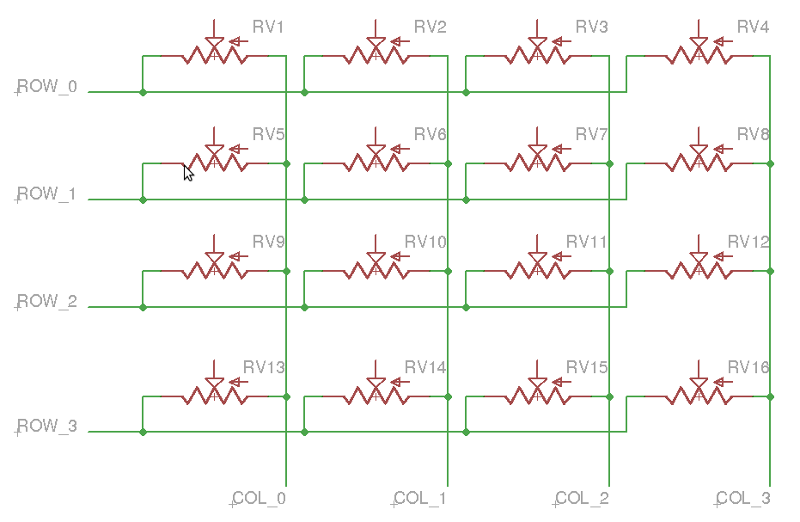
\includegraphics[width=\columnwidth]{figures/matrix}
    \caption{Illustration of a part of the variable "resistor" matrix for 3d pressure sensing.}\label{fig:matrix}
\end{figure}



\subsection{Sensor Control}
\subparagraph{Microcontroller}

We use a Teensy 3.x\footnote{\url{http://pjrc.com/teensy}} to sample the voltages of the sensor. Due to the large number of analog inputs the Teensy allows us to read all 16 voltages without adding any external hardware.
The measured voltages are converted and sent as data packets to a computer. Additionally, we use the analog output of the Teensy to generate audio based on the sampled voltages, this allows the Musical Skin to be used without tethering it to a computer.

\subparagraph{Computer}
When connected to a computer by USB, the raw data output is processed by an open frameworks\footnote{\url{http://openframeworks.cc}} program. We initially interpolate the raw position data as this improves the localization of touches spanning multiple strips. We use blob detection algorithms from OpenCV\footnote{\url{http://opencv.org}} to detect the size and locations of touch points. Each blob's centroid and pressure level can be sent to other applications such as Ableton Live using the OSC protocol. This enables the Musical Skin to control a music applications or interactive visualizations as will be demonstrated during the exhibition.


\section{The Installation}
The installation can be adopted to the constraints and opportunities of the space available to us. We envision an enclosed and dimly lit space that contains our Skins. Visitors will enter this space and see our fabric instruments illuminated. The slight illumination of the fabric is intended to invite people to touch it. Once they do, the room will light up softly. Each fabric instrument makes the room light up in different ways, each fabric instrument has its own colors.

Visitors will discover that different instruments have different sound qualities. Some instruments will allow for expressive pressure based interactions triggering ambient pads and soundscapes, others can be played much like a harmonic keyboard. Others again will trigger one-shot sounds, enabling percussive sounds and drumming. The soft malleable nature of the instruments allows for interesting explorations not possible with conventional interfaces. For example, while a single touch typically would trigger a single sound or drum hit, if the instrument is folded, visitors can create custom polyphonic soundscapes. Visitors can explore rubbing, rolling, crumbling to create chaotic or non-deterministic sounds, or lay it out flat on an even surface for high-detail interaction.

Our instruments can be draped over objects to create custom shaped instruments. We will bring a small number of wooden and cardboard shape-primitives that can be used for this purpose. An e-textile might be wrapped around a cylindrical object for providing a better grip, or laid out over a concave bowl to allow faster motion between different areas. Different shapes provide different musical affordances.

Finally our instruments can be draped over bodies. This allows us to use our own bodies as instruments: we can amplify body percussion with additional sounds, or we can hug each other to create soundscapes. The ability to drape these instruments over our body allows us to explore what interactive tattoos might feel like, or what other methods of input in soft fabric devices might feel like on the body. Finally it also allows visitors to explore interacting with interfaces on other peoples bodies. This type of expressive on-body input is something that we have very little experience with and this will allow visitors to improve their intuitive understanding of such potential technologies.


\section{Limitations and Future Work}

\begin{figure}[!h]
    \centering
    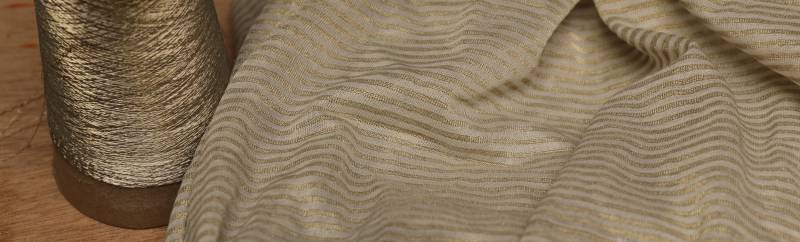
\includegraphics[width=\columnwidth]{figures/zebra_fabric}
    \caption{The new custom made conductive fabric.}\label{fig:zebra_fabric}
\end{figure}

While the sensor has a very high resolution along the pressure axis, the spatial resolution is limited by the materials and sensing approach. The minimum spacing between individual sensing strips is constrained by the fabrics we use. We have not established the minimum size yet, but anticipate that there will be a material constrained limiting the resolution.
Having said that, we have found that software interpolation works quite well, as usually more than one sensing strip is touched at once. We hope to further improve the software filtering by to using trajectory prediction algorithms such as Kalman filters used in the LumoSpheres project \cite{lumospheres}.

On the conductive fabric side, there are improvements possible using custom woven fabric with integrated conductive strips. Doing so may increase the sensors resolution and robustness. Figure \ref{fig:zebra_fabric} shows a first attempt at this.

The sensing approach also requires a large number of analog inputs on the micro-controller side. Currently the maximum resolution we can obtain is a matrix of 16 by 16. When we create larger fabric, they do not have a higher resolution, as they still use the 16 by 16 sensing strip design. We are current working on a dedicated micro-controller circuit to improve this.

Finally, we are interested in adding actuation for haptic feedback. We have experimented with "analog" solutions using thick ink to infer finger position and motion on the sensor (see \ref{fig:zoom}), but we hope to find an active solution in the future.
We have investigated using previous experimentations such as BubbleWrap \cite{bubblewrap} or Shade Pixel \cite{shadepixel} however this added too much bulk to the fabric. While we still wish to add haptic feedback, more experimentation is required to decide on a best approach for this.

\begin{figure}[h!]
    \centering
    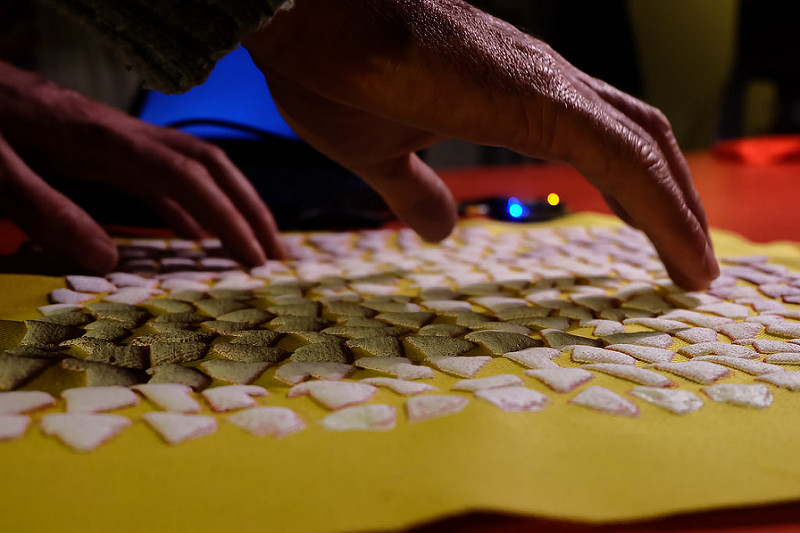
\includegraphics[width=\columnwidth]{figures/zoom}
    \caption{Illustration of an "analog" haptic feedback experimentation.}\label{fig:zoom}
\end{figure}

\section{Conclusion}
We suggest an installation consisting of three soft fabric instruments which can be used by visitors to control the environment in the form of adapting sound and lighting. The primary intent of the fabric instruments is for collaboratively making music while exploring shapes, materiality and bodies. This can be done by draping the fabric over objects, folding and deforming the fabric, or wearing it on the body. The e-textile itself is open source and improves over similar sensing applications both in terms of robustness and resolution. We are submitting this installation both because we believe it matches the theme of this years art exhibition, and because we believe it will be an engaging experience for people interested in the topics of TEI.


% \balance{}

\bibliographystyle{SIGCHI-Reference-Format}
\bibliography{tei17}

\end{document}

%%% Local Variables:
%%% mode: latex
%%% TeX-master: t
%%% End:
